\chapter{Results}\label{chap:results}

The following section describes the experimental setup, the used datasets and parameters and the experimental results achieved.

\section{Developped programs}
Many programs have been developped for the need of the present thesis. Early data exploration scripts have paved the way towards efficient highly parallel programs in both Rust and Python for data analysis, graph and embedding generation of ML and DL tested on different models and contexts. All the necessary concepts and methods have been introduced previously, so it is now time to present those main program in details.

\subsection{Mem2Graph}

\subsection{Machine Learning pipelines}

\section{Experimental Setup}
The following section dwelves deeper into the experiment setup and the experiments that have been conducted at large scale, on the server. It includes some selected program output logs to give precise details about the program parameters, environment and usage. 

All those elements are not for mere Illustration but give invaluable insights and allows to support the discussion of the challenges encountered, specifically during the large scale experiments.

The final experiments were conducted following those steps:

0. Cleaning the original Zenodo dataset into a cleaned RAW heap dump dataset
1. Generating graphs with their embeddings using the Mem2Graph Rust program. A python launcher script allows to easily generate several memgraph dataset with different combination of program params
2. Using a sanity check Python program for data preloading and data validation
3. Running the ML and DL GCN pipelines with the main Python program. This program is responsible for easi launching of the data science, machine learning training and model evalution launching, and is able to cover a predefined range of parameters and model hyperparameters.
4. Result collection, evaluation, visualization and error handling with eventual corrections to prepare for next iteration and confront hypotheses and research questions

\subsection{Generation of the memgraph datasets}
Using Mem2Graph, 

\subsection{Working with a huge dataset}

* 26202 RAW heap dump files in the pre-cleaned dataset
* With Mem2Graph, we focus on 3 custom embeddings. For each of those embeddings, we can choose to add the additional filtering feature discussed earlier. This gives us 6 Mem2Graph output dataset generation, each containing 26202 memgraph files containing graphs with custom node embeddings.

Loading the graph from DOT files into NetworkX graph in Python is a ressource intensive operation that consumes all the available computing power on all tested platforms (laptop, servers). It takes several dozens of seconds to load a memory graph. It has been experimented that saving those loaded graphs using the \textit{pickle} python library allows to perform checks while loading the graph, add more information about each graph. 

Dealing with many files was a source of errors. So to verify the memory graph dataset generation as well as transforming DOT files into pre-saved networkx graph, a sanity checking script has been developed.




Below is a sample of the logs generated by the sanity check script:

\begin{lstlisting}[language=bash, caption={Result logs of the \texttt{memory\_graph\_gcn/src/sanity\_check\_gv\_files.py} program.}, literate={_}{\_}{1}]
    * Running program...
   Passed program params:
   param[0]: src/sanity_check_gv_files.py
   param[1]: -k
   Parsed program params:
   keep_old_output: True
   skip_dir_starting_with_number: None
   dry_run: False
    * Now, performing data loading and sanity checks...
    * Looking for Mem2Graph dataset directories in /root/phdtrack/mem2graph/data...
    * Skipping .gitignore...
    * Found 6 Mem2Graph dataset directories.
   Mem2Graph dataset dir paths:
    -> /root/phdtrack/mem2graph/data/0_graph_with_embedding_comments_-v_-a_chunk-header-node_-c_chunk-semantic-embedding_-e_none_-s_none, which contains 26202 files.
    -> /root/phdtrack/mem2graph/data/1_graph_with_embedding_comments_-v_-a_chunk-header-node_-c_chunk-statistic-embedding_-e_none_-s_none, which contains 26202 files.
    -> /root/phdtrack/mem2graph/data/2_graph_with_embedding_comments_-v_-a_chunk-header-node_-c_chunk-start-bytes-embedding_-e_none_-s_none, which contains 26202 files.
    -> /root/phdtrack/mem2graph/data/3_graph_with_embedding_comments_-v_-a_chunk-header-node_-c_chunk-semantic-embedding_-e_only-max-entropy_-s_activate, which contains 26202 files.
    -> /root/phdtrack/mem2graph/data/4_graph_with_embedding_comments_-v_-a_chunk-header-node_-c_chunk-statistic-embedding_-e_only-max-entropy_-s_activate, which contains 26202 files.
    -> /root/phdtrack/mem2graph/data/5_graph_with_embedding_comments_-v_-a_chunk-header-node_-c_chunk-start-bytes-embedding_-e_only-max-entropy_-s_activate, which contains 26202 files.
    * Loading graphs in /root/phdtrack/mem2graph/data/0_graph_with_embedding_comments_-v_-a_chunk-header-node_-c_chunk-semantic-embedding_-e_none_-s_none...
   [...]
   Loading graphs: 100%|##########| 26201/26202 [3:22:17<00:00,  1.17it/s]
   Loading graphs: 100%|##########| 26202/26202 [3:22:25<00:00,  3.19s/it]
   Loading graphs: 100%|##########| 26202/26202 [3:22:25<00:00,  2.16it/s]
    * Checking embedding length of graphs in /root/phdtrack/mem2graph/data/5_graph_with_embedding_comments_-v_-a_chunk-header-node_-c_chunk-start-bytes-embedding_-e_only-max-entropy_-s_activate...
   -> [x] 26202 graphs in /root/phdtrack/mem2graph/data/5_graph_with_embedding_comments_-v_-a_chunk-header-node_-c_chunk-start-bytes-embedding_-e_only-max-entropy_-s_activate have been loaded and checked.
   -> [_] 0 graphs in /root/phdtrack/mem2graph/data/5_graph_with_embedding_comments_-v_-a_chunk-header-node_-c_chunk-start-bytes-embedding_-e_only-max-entropy_-s_activate have been skipped (deleted).
   [x] 157212 total graphs in the input mem2graph dataset dir paths have been loaded and checked.
   [_] 0 total graphs in the input mem2graph dataset dir paths have been skipped (deleted).
   <END> Program took: 42626.062309 total sec (11h 50m 26s)
\end{lstlisting}

\subsection{Dealing with hyperparameter tuning}

\subsection{The challenge of ressource optimisation}

\subsection{The challenge of packet management}

\section{Obtained results on feature engineering}

\begin{lstlisting}[language=bash, caption={Command used to count the number of .gv memory graph files generated by \textit{mem2graph} inside one of the servers mem2graph dataset directory.}]
    (py311) root@compute-container-rascoussie-d584d4794-lbm9r:~/onyr_phdtrack/mem2graph# find data/ -type f -name "*.gv" | wc -l
    104808
\end{lstlisting}

\section{Feature Engineering results}

\begin{figure}[H]\label{results:corr_matrices:kendall}
    \centering
    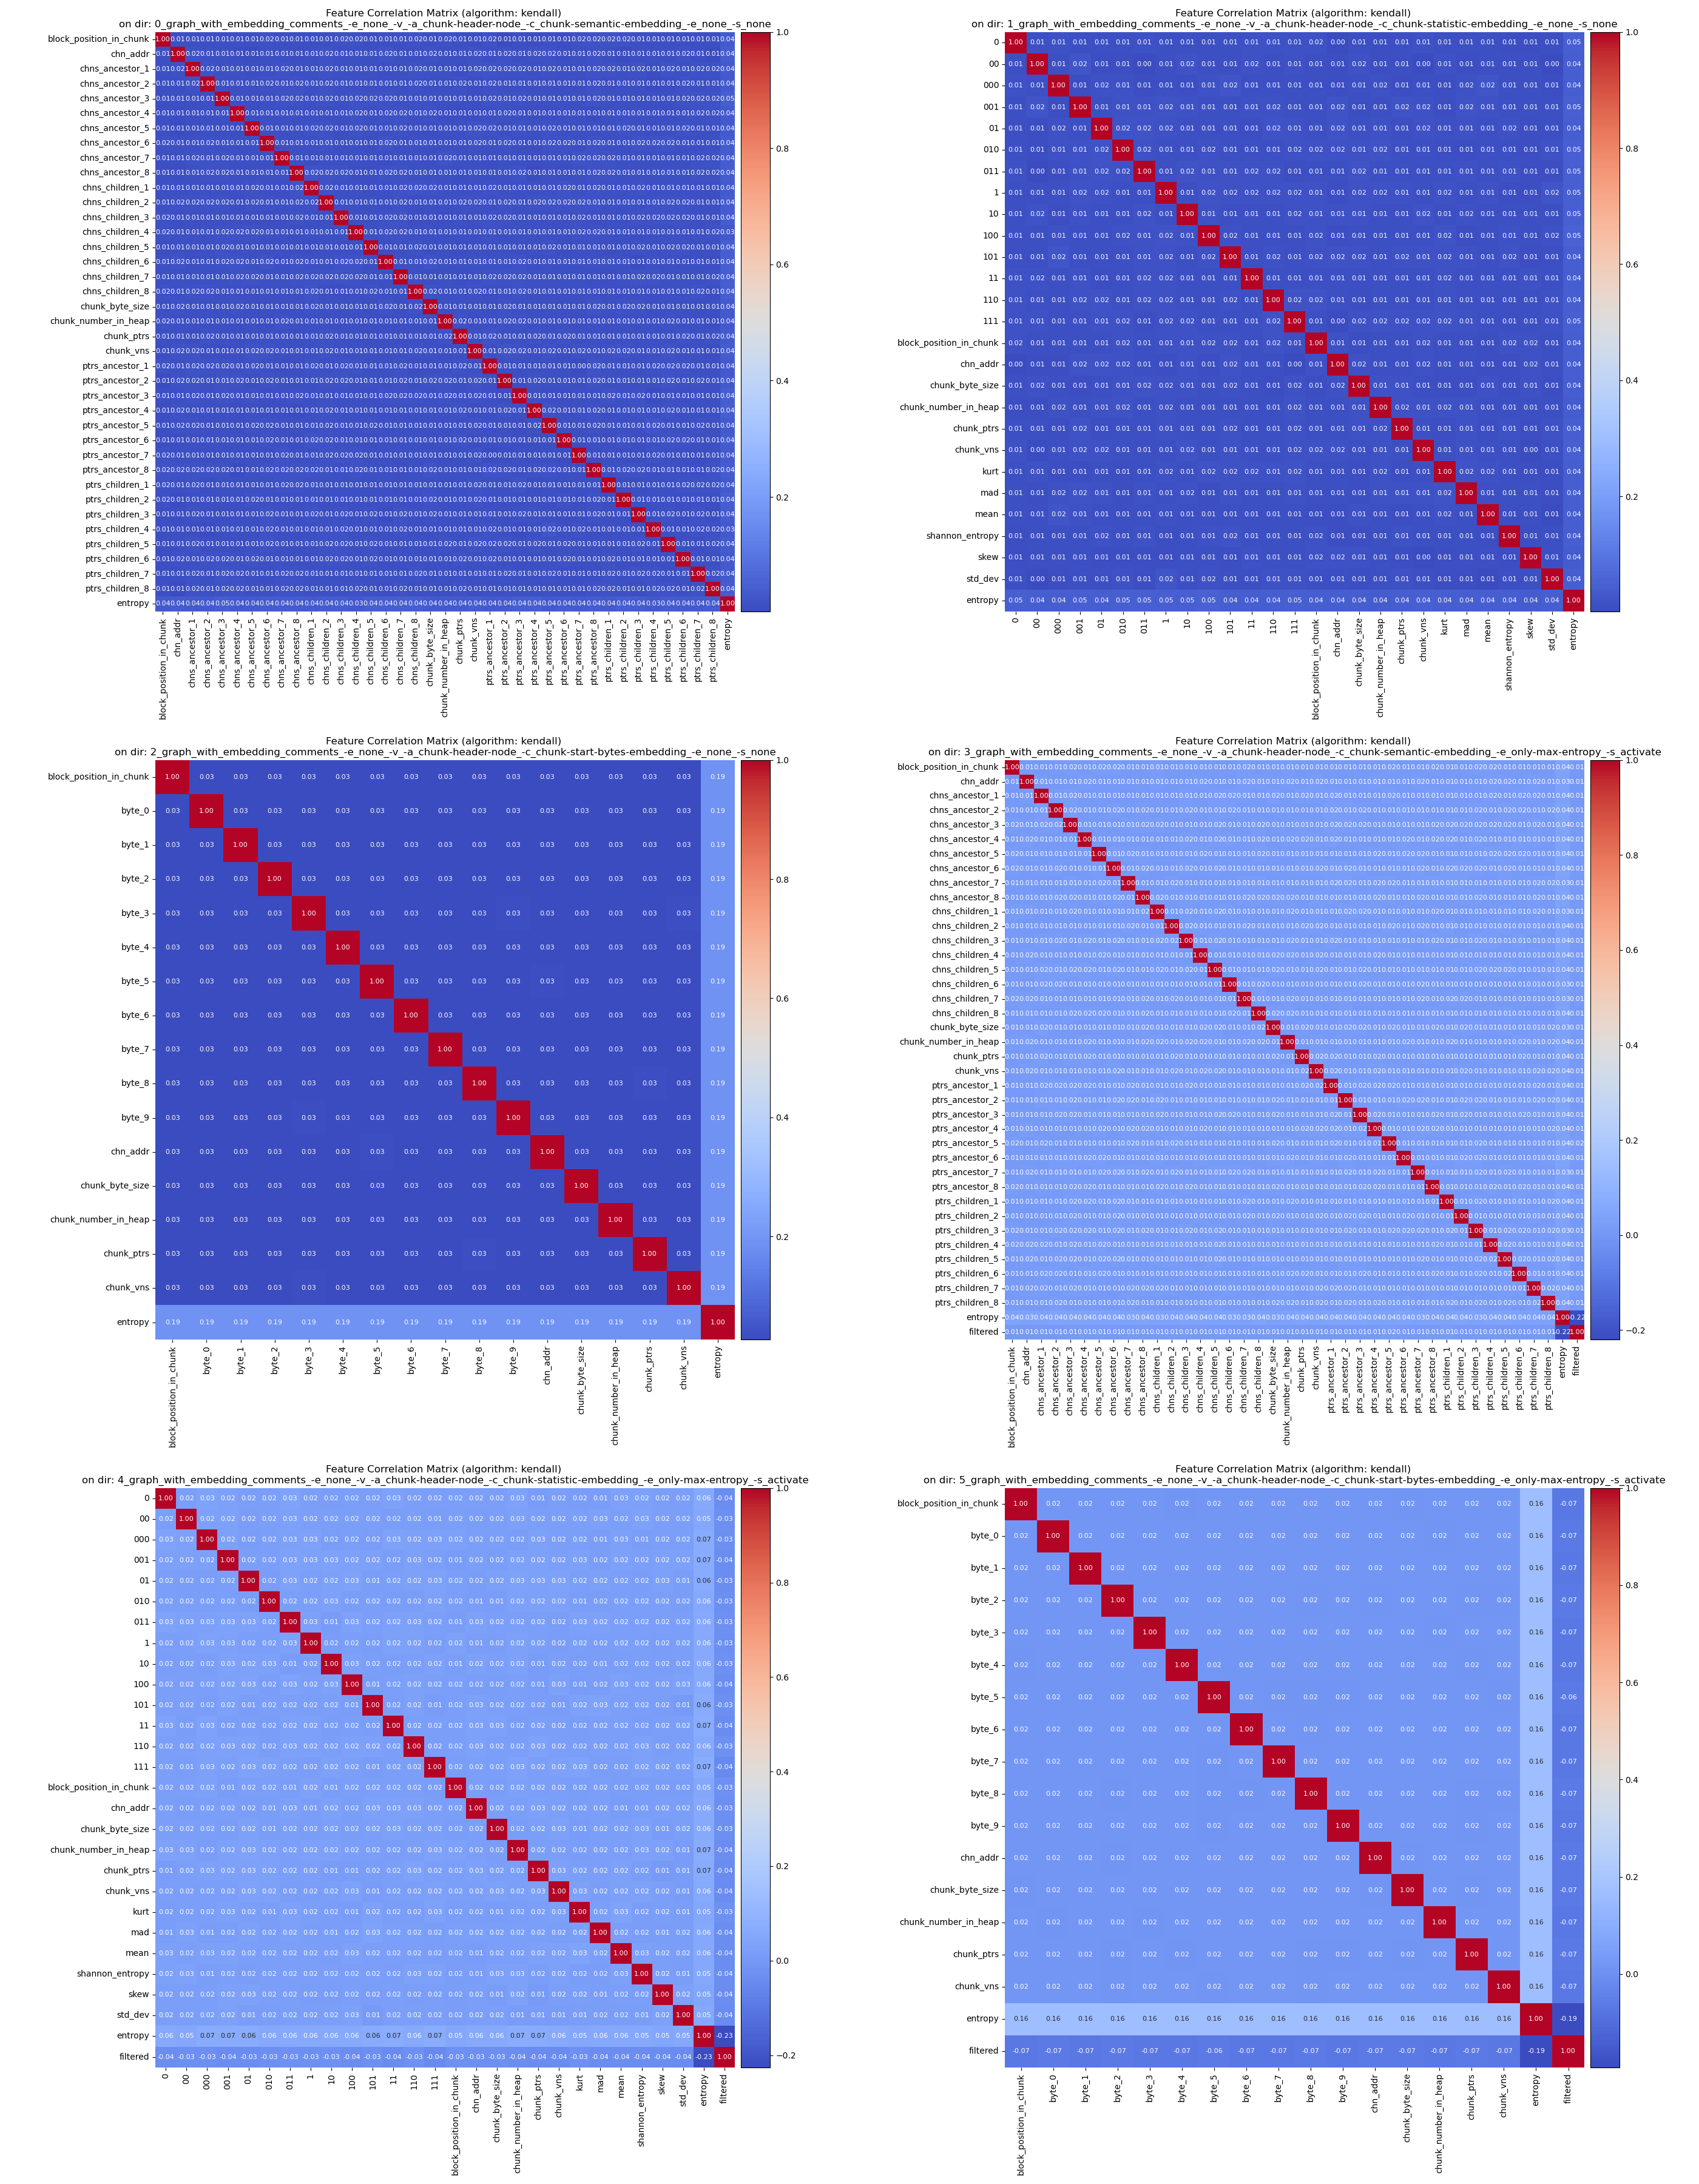
\includegraphics[width=16cm]{feature_engineering/concatenated_1_2023_10_24_kendall.png}
    \caption{Feature correlation matrices on the different Mem2Graph-generated datasets. Used algorithm: Kendall.}
\end{figure}

\begin{figure}[H]\label{results:corr_matrices:pearson}
    \centering
    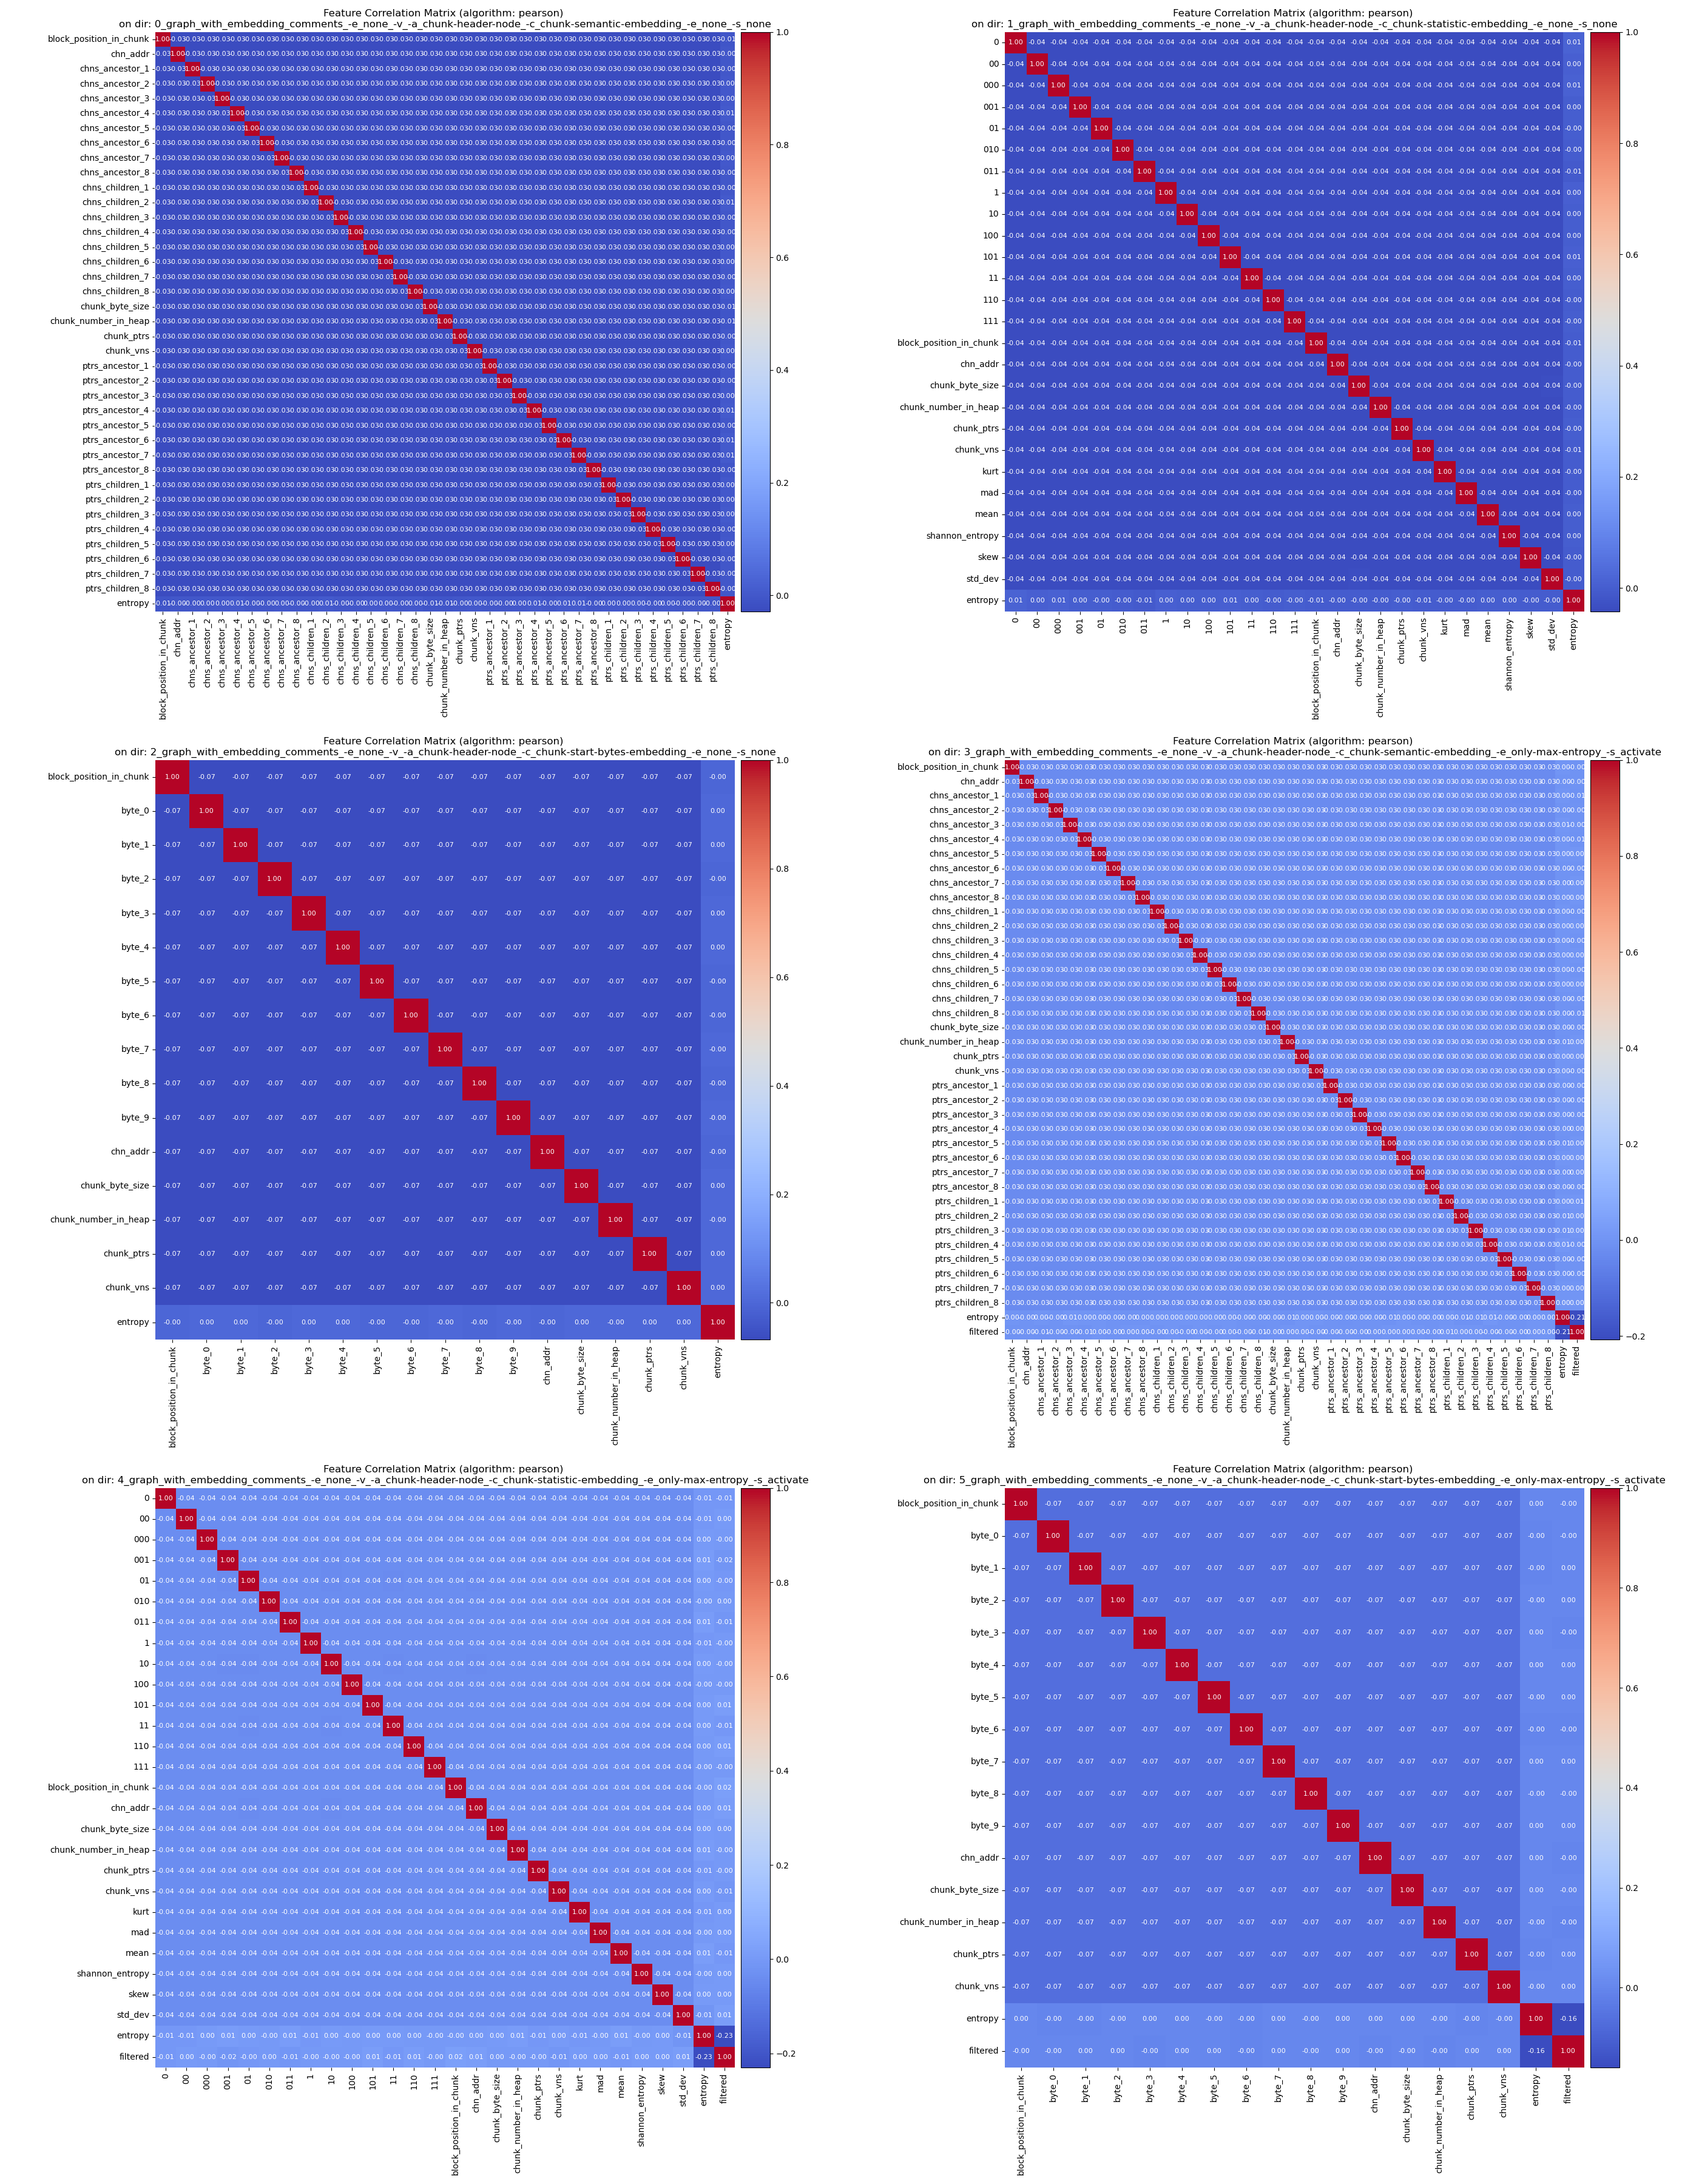
\includegraphics[width=16cm]{feature_engineering/concatenated_2_2023_10_24_pearson.png}
    \caption{Feature correlation matrices on the different Mem2Graph-generated datasets. Used algorithm: Pearson.}
\end{figure}

\begin{figure}[H]\label{results:corr_matrices:spearman}
    \centering
    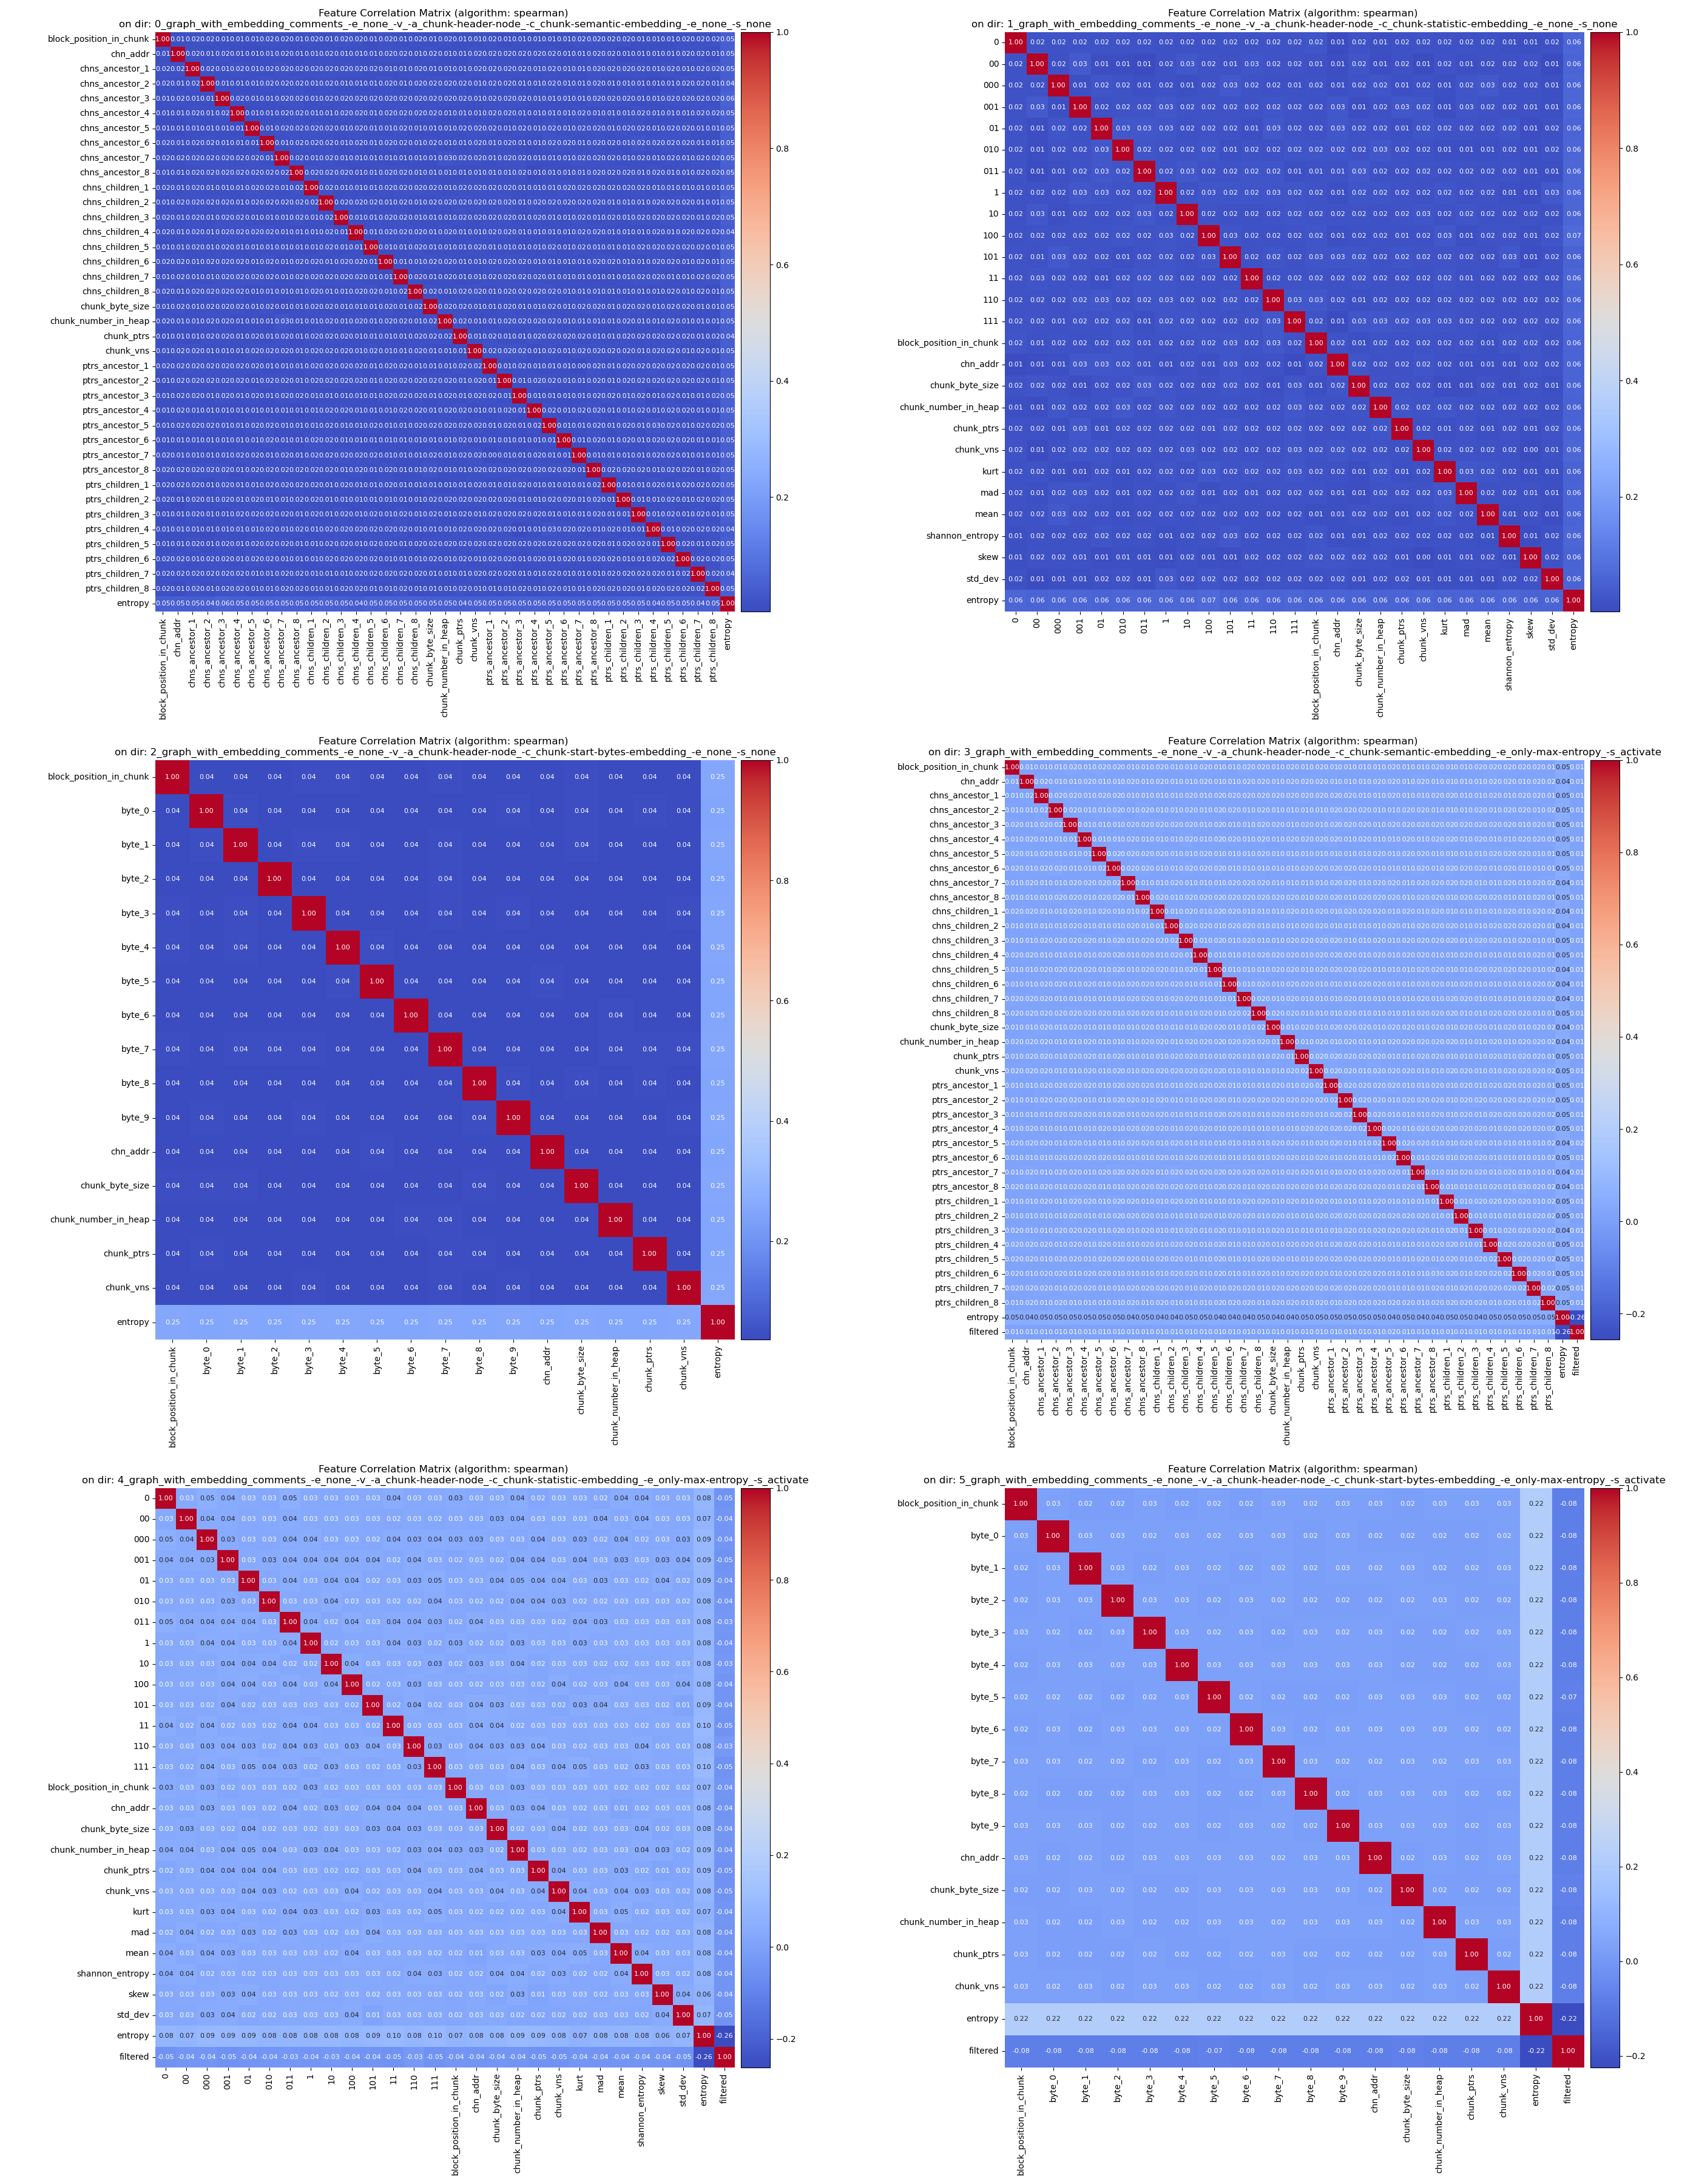
\includegraphics[width=16cm]{feature_engineering/concatenated_3__2023_10_24_spearman.png}
    \caption{Feature correlation matrices on the different Mem2Graph-generated datasets. Used algorithm: Spearman.}
\end{figure}

\section{Classic Model results}

\section{Deep Learning Model results}


\section{Comparing performances of models and embeddings}
* Comparing all computed results, on a maximum number of input graph of 16, which is really low. This is due to the fact that we have so many hyperparameters, embeddings and models to compare.
* Results on 7976 machine learning pipelines, for a cumulated compute time of over 100h.

\begin{figure}[H]\label{results:compare:models:full}
    \centering
    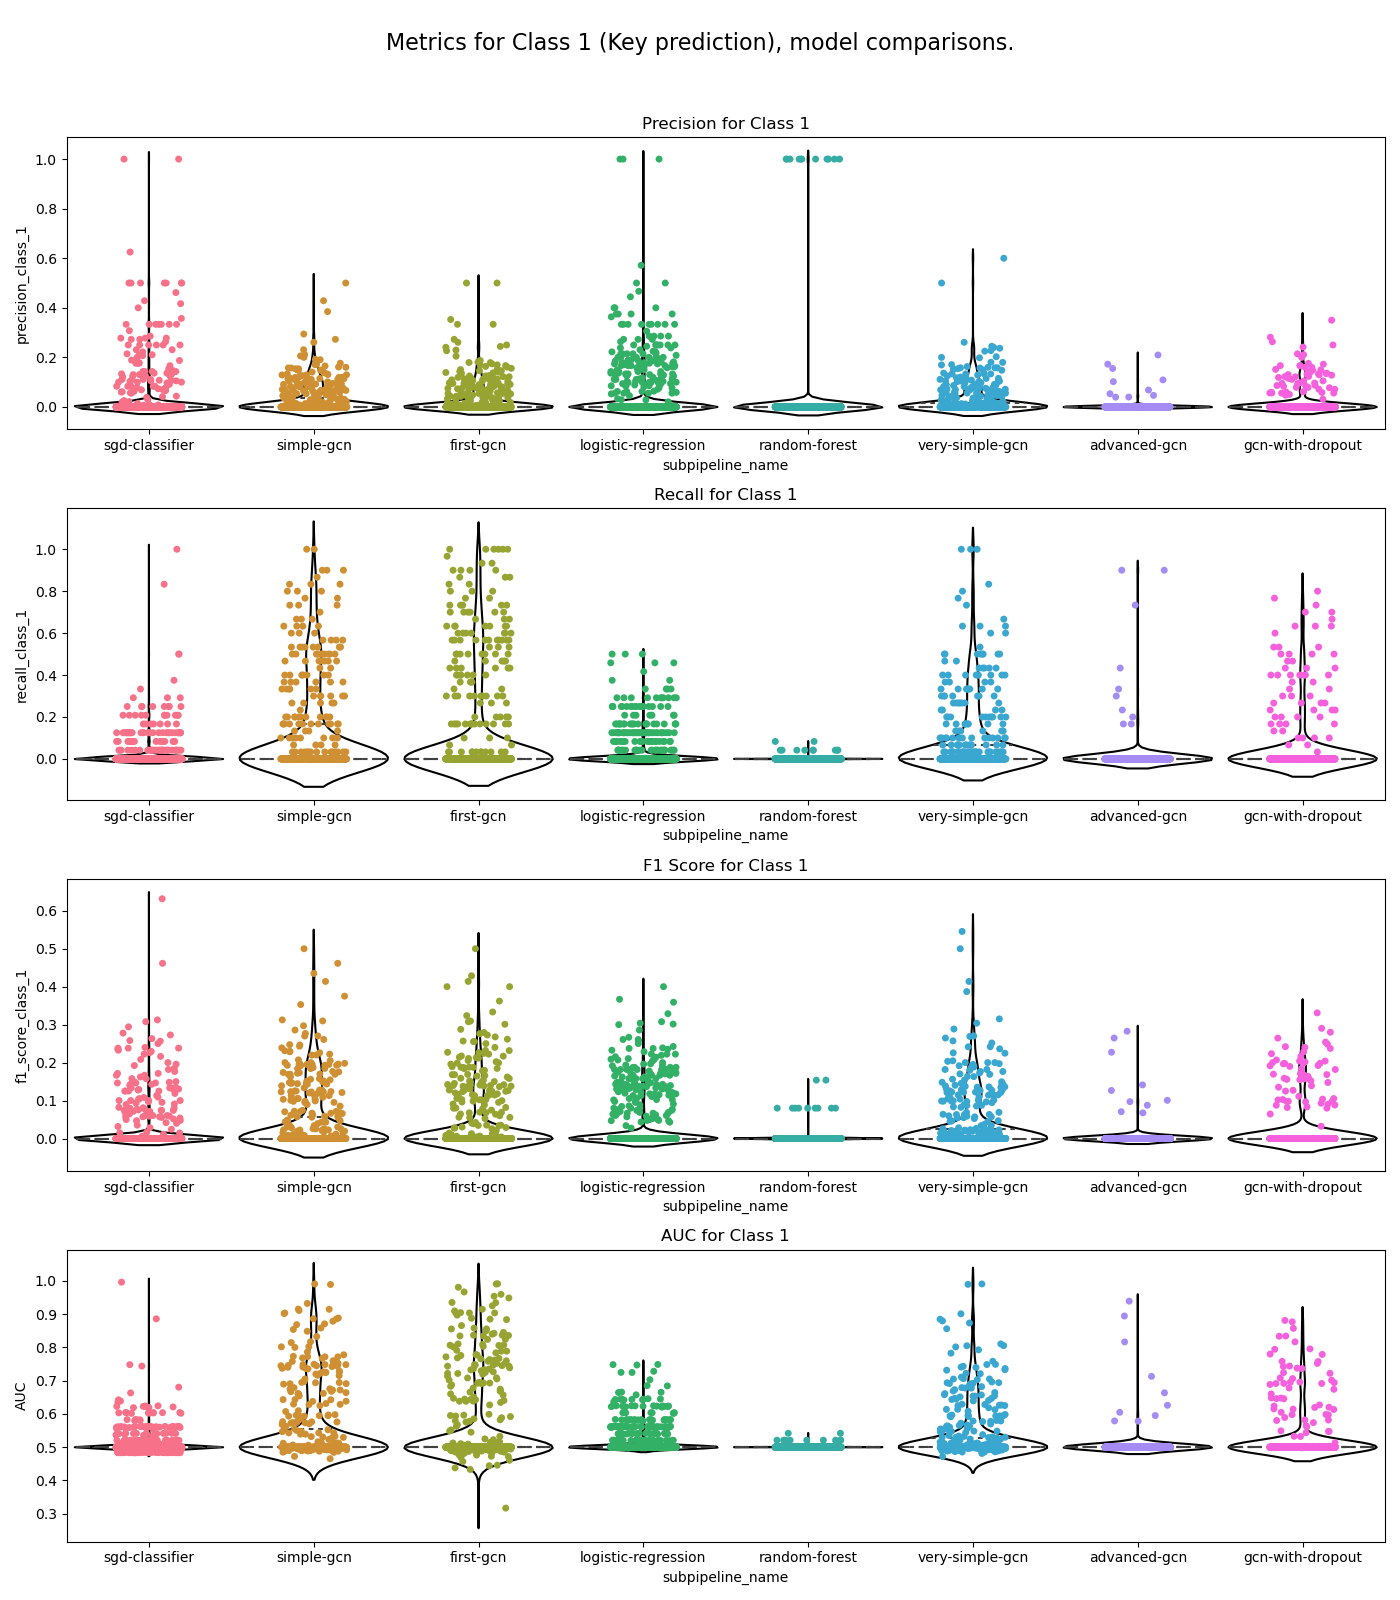
\includegraphics[width=16cm]{plots/models_comparison_metrics.png}
    \caption{Visualization of the result metrics use to compare model performance on memory graphs, for different embeddings and hyperparameters.}
\end{figure}

\begin{figure}[H]\label{results:compare:embeddings:full}
    \centering
    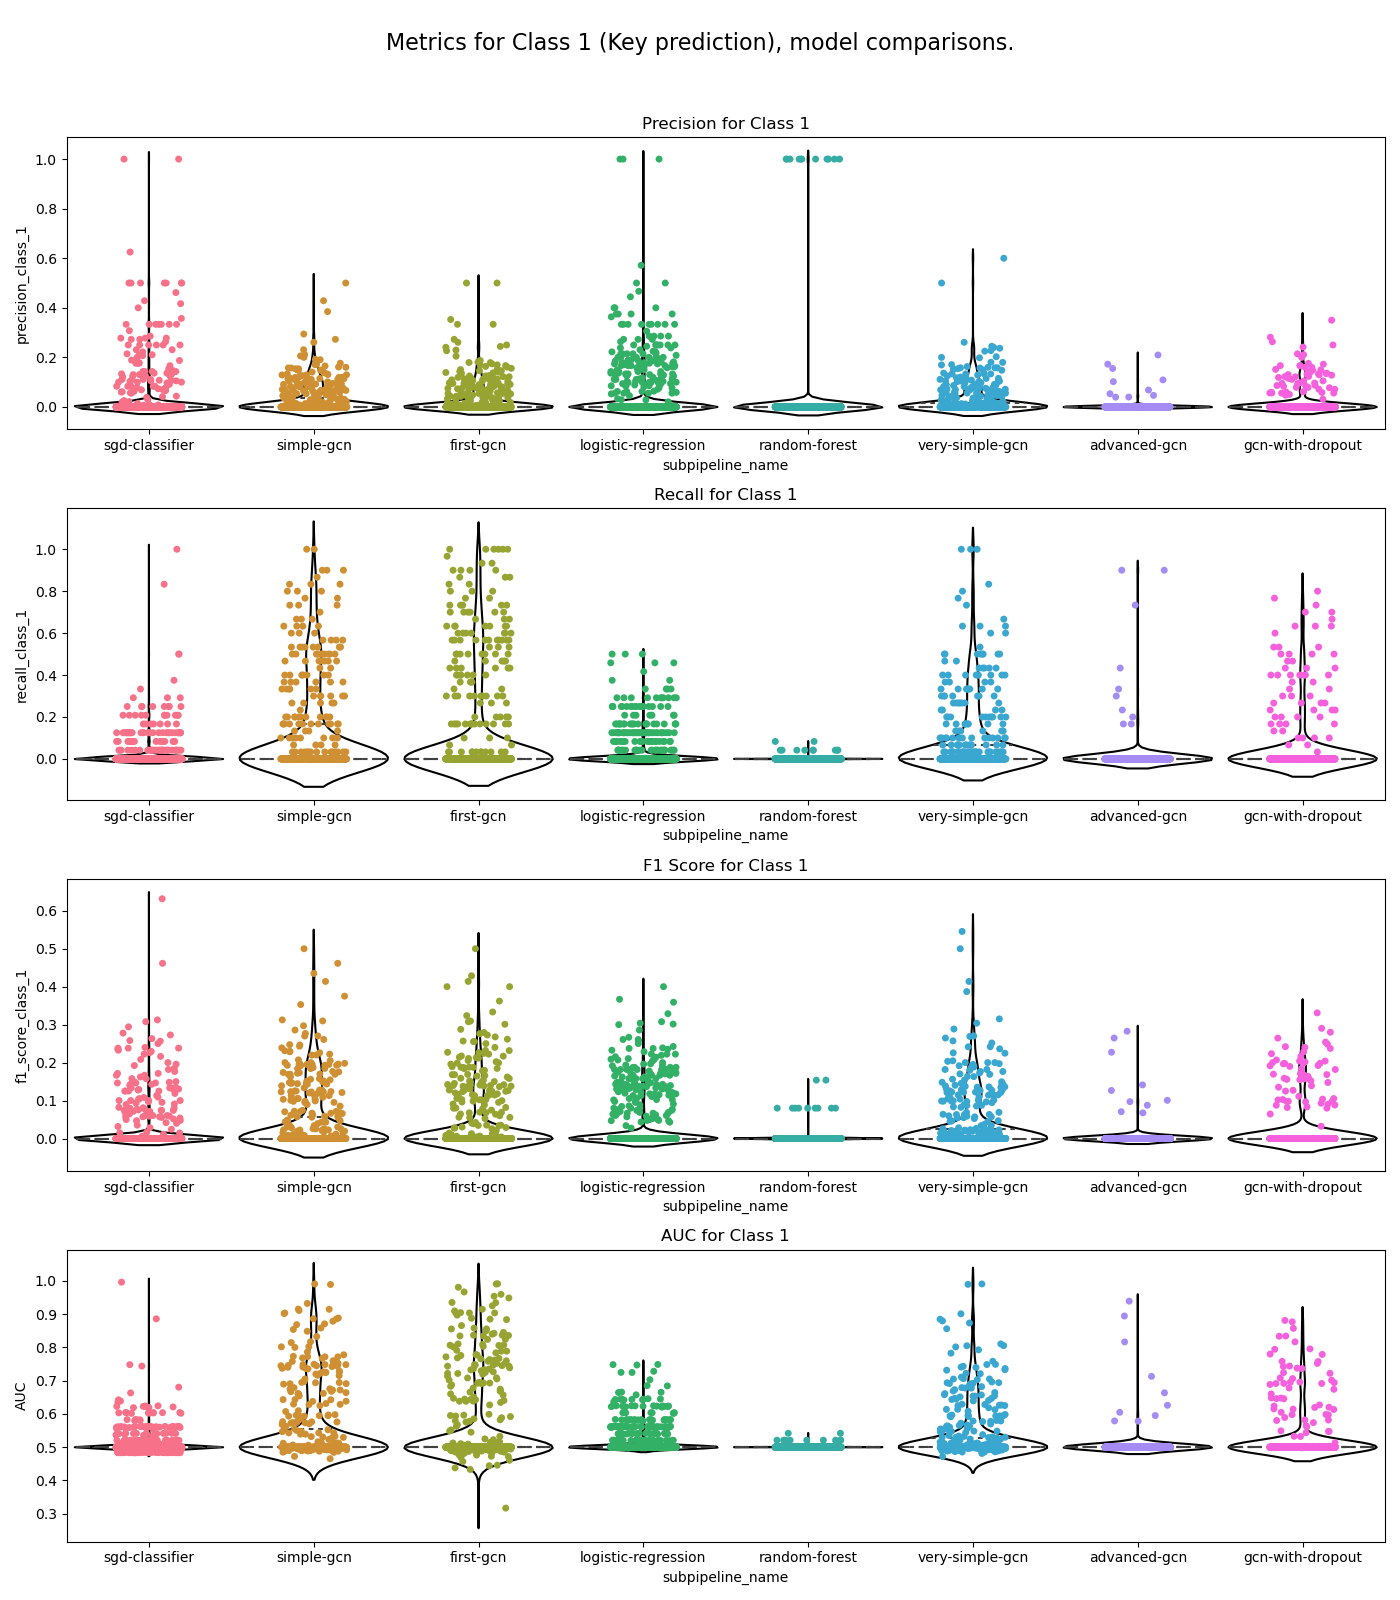
\includegraphics[width=16cm]{plots/models_comparison_metrics.png}
    \caption{Visualization of the result metrics use to compare model performance per memory graph node embedding strategies.}
\end{figure}


